\documentclass{beamer}

\usepackage[utf8]{inputenc}
\usepackage{eurosym}
\usepackage{hyperref}
\hypersetup{
    colorlinks = true
    }
\usepackage{graphicx}

%Information to be included in the title page:
\title{GTA Einführung Robotik mit Makecode}
\author{Mattias Schlenker}
\institute{Wilhelm-Ostwald-Gymnasium}
\date{28. Januar 2021}

\begin{document}

\frame{\titlepage}

\begin{frame}
\frametitle{Spannender mit schießendem Gegner}

Damit ein Gegner schießen kann, muss ,,das Spiel'' immer seien Position kennen. Das geht mit einer globalen Variablen, die ein Sprite enthält und in der Startroutine initialisiert wird:
 
 \begin{figure}
  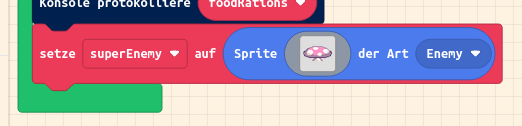
\includegraphics[width=8cm]{game19.png}
  \caption{Globale Variable}
  \label{fig:game19}
\end{figure}

\end{frame}

 \begin{frame}
 \frametitle{Nur initialisieren, nicht anzeigen!}
 
 Vor dem Start initialisierte Sprites werden in der Bildschirmmitte angezeit, würden also sofort mit dem Spielerraumschiff kollidieren. Als kleinen Workaround platzieren wir das Sprite am unteren Rand und zerstören es sofort: 
 
 \begin{figure}
  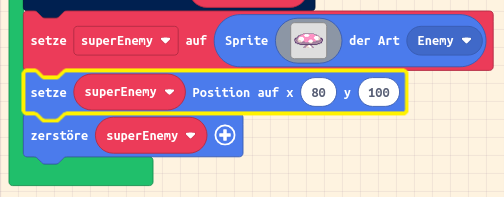
\includegraphics[width=8cm]{game20.png}
  \caption{Sprite wird sofort zerstört}
  \label{fig:game20}
\end{figure}

\end{frame}

 \begin{frame}
 \frametitle{Super-Gegner ins Spiel bringen}
Wichtig ist es, nur einen Gegener im Spiel zu haben. Dafür prüfen wir einfach, ob die Y-Position des Gegners im Bereich zwischen 1 und 100 liegt. Ist das nicht der Fall, wird der Super-Gegner wie jeder andere Gegner initialisiert, bekommt aber eine eigene Klasse zugeordnet:

 
 \begin{figure}
  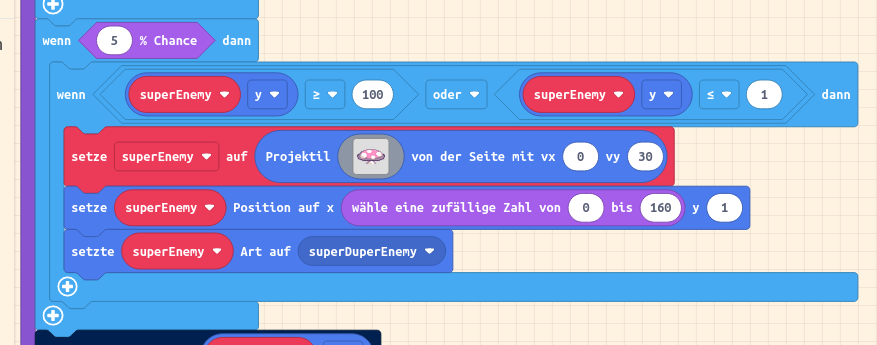
\includegraphics[width=8cm]{game21.png}
  \caption{Super-Gegner ins Spiel bringen}
  \label{fig:game21}
\end{figure}
\end{frame}

 \begin{frame}
 \frametitle{Super-Gegner schießt}
Um zu schießen, muss zunächst geprüft werden, ob überhaupt ein Super-Gegner sichtbar ist. Ist das der Fall, wird an der Position des Super-Gegners ein Projektil erzeugt, dessen Geschwindigkeit etwas größer ist als die des Super-Gegners: 
 \begin{figure}
  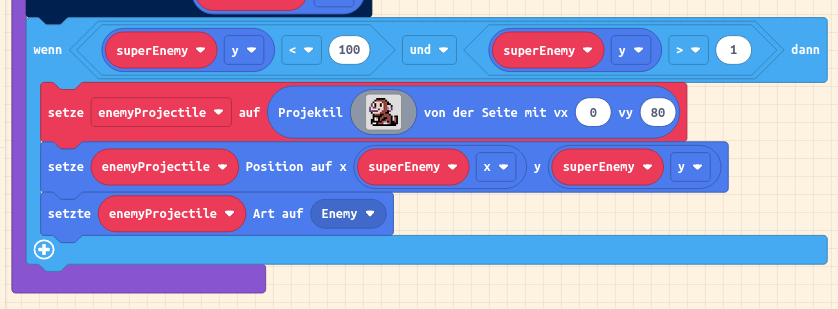
\includegraphics[width=8cm]{game22.png}
  \caption{Vom Super-Gegner ausgehendes Projektil}
  \label{fig:game22}
\end{figure}
\end{frame}


 \begin{frame}
 \frametitle{Super-Gegner abschießen}
Beim Abschießen ist zu beachten, dass die Zerstörung des Sprites dieses zwar aus dem Spiel entfernt, das Objekt selbst aber noch initialisiert ist und die X- und Y-Position zum Zeitpunkt des Abschusses behält. Als Workaround setzen wir das Super-Gegner-Sprite unmittelbar vor der Zerstörung an den oberen Bildschirmrand. 
 
 \begin{figure}
  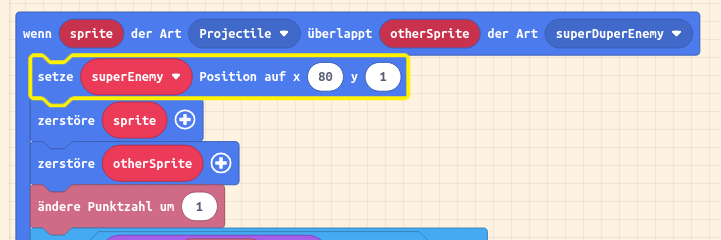
\includegraphics[width=8cm]{game23.png}
  \caption{Erst positionieren, dann zerstören}
  \label{fig:game23}
\end{figure}
\end{frame}

 \begin{frame}
 \frametitle{Feinarbeit}

Die Kollisionserkennung ist identisch zum Crash mit normalen Gegnern. Überlegt selbst, ob Ihr die gegnerischen Projektile abschießbar macht. Etwas hübscher wird es, wenn Ihr die gegnerischen Projektile nicht an der Y-Koordinate erzeugt, sonder einige Pixel draufpackt. Als weitere Erweiterung ist denkbar, dass der Gegner Eurer Position folgt, also eine geringe vX setzen, je nachdem, ob Ihr Euch rechts oder links von ihm befindet. 

Beispielcode dieser Session: \href{https://makecode.com/\_io5V94K01Vvw}{https://makecode.com/\_io5V94K01Vvw} oder als UF2 in LernSax

\end{frame}

\end{document}
